\documentclass[11pt]{article}

\usepackage[brazil]{babel} 
\usepackage[latin1]{inputenc} 
\usepackage{alltt}
\usepackage{multicol} 
\usepackage{graphicx}
\usepackage{listings}

\setlength{\topmargin}{-2.5cm} 
\setlength{\textheight}{26.5cm}
\setlength{\oddsidemargin}{-2cm} 
\setlength{\evensidemargin}{-2cm}
\setlength{\textwidth}{7.5in}

\newcommand{\comb}[2]
%%  to be used in math mode 
{\left( \begin{array}{c} #1 \\ #2 \end{array} \right) }
 
\def\ni{\noindent}

\def\idc{\makebox[1.5cm]{}}

\def\espaco{\makebox[5mm]{}}
 
\def\ua{\uparrow}
 
\def\pule{\vspace{0.2cm}} \def\pulao{\vspace{0.5cm}}
 
\newcommand{\primeira}[1] {$#1^{\mbox{\scriptsize\b{a}}}$}
 
\newcommand{\primeiro}[1] {#1$^{\mbox{\scriptsize\b{o}}}$}
 
\begin{document}
\lstset{language=Java}
\lstset{frameround=fttt}
\thispagestyle{empty}
\begin{center}

\hfill {\small Departamento de Computa��o -- Universidade Federal de S�o Carlos}
       \\
\hspace{1cm}\\

  \textbf{\large 1001507 - PROGRAMA��O ORIENTADA A OBJETOS}

  \textsc{Professor: Delano M. Beder}

\end{center}

\section*{Enunciado}

A atividade consiste em implementar (em  C++) as  classes conforme as instru��es fornecidas abaixo:

\vspace{0.5cm}

% Obs: Organize suas classes no {\it namespace} {\bf poo}

% \vspace{0.5cm}

%\begin{figure}[htb]
%\centering\includegraphics[width=8cm]{2}
%\label{ArqFig}
%\end{figure}

\begin{enumerate}


\item Defina a classe {\sf Pessoa}  com os seguintes atributos: {\sf nome} (tipo
  {\bf string})  e {\sf  CPF} (tipo  {\bf inteiro}).

 Inclua na classe: (a)  um construtor �nico capaz de setar  os atributos (nome e
 CPF),  (b)  os m�todos  {\it  getters}  e (c)  o  m�todo  {\sf void  imprime()}
 respons�vel pela impress�o das informa��es de uma pessoa.

\item Defina a classe {\sf Professor}, subclasse da classe {\sf Pessoa} definida
  na  quest�o  1,  e que  possui  o  atributo  {\sf  sal�rio} (tipo  {\bf  ponto
    flutuante}).

\begin{itemize}

\item Inclua  na classe  um construtor  �nico capaz  de setar  os atributos  e o
  m�todo {\sf void  imprime()} respons�vel pela impress�o das  informa��es de um
  professor.

\item Implemente os m�todos {\it getters} nessa classe.

\end{itemize}

\item Defina  a  classe  {\sf Coordenador},  subclasse  da  classe  {\sf
  Professor} definida  na quest�o 2, e  que possui o atributo  {\sf curso} (tipo
  {\bf string}) que representa o curso que esse professor coordena.

\begin{itemize}

\item Todo professor coordenador recebe uma bonifica��o adicional de R\$ 2000,00
  devido o cargo que ocupa. Dessa forma, redefina o m�todo {\sf getSal�rio()} de
  tal forma que retorne o sal�rio do coordenador (com a bonifica��o inclusa);

\item Inclua  na classe  um construtor  �nico capaz  de setar  os atributos  e o
  m�todo {\sf void  imprime()} respons�vel pela impress�o das  informa��es de um
  coordenador.
  
\end{itemize}

\end{enumerate}

\hspace{1cm}\\

\centering
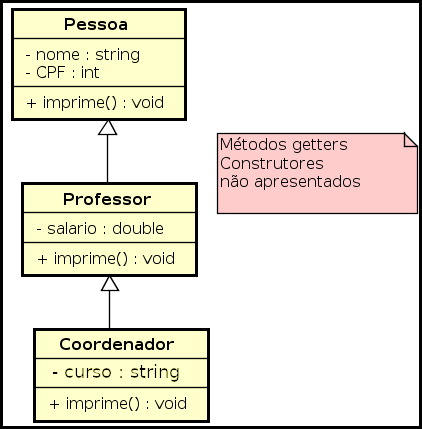
\includegraphics[width=8cm]{classes.png}

\end{document}
